% ══════════════════════════════════════════════════════════════════════════════
%  CAPITOLO — DATI E COSTRUZIONE DEL DATASET
%  Etichette: ch:data, sec:rawdata, sec:decisioni, sec:cleaning, sec:phaselog,
%             sec:dataset, sec:datasummary
%             tab:files, tab:colmap, tab:nulli_sede, tab:cleaninglog, tab:columns
% ══════════════════════════════════════════════════════════════════════════════

\chapter{Dati originali e Costruzione del Dataset}
\label{ch:data}

Il presente capitolo descrive il materiale empirico su cui poggia l'intero
elaborato: la provenienza e la struttura dei file grezzi forniti dal
Dipartimento Interaziendale di Medicina Trasfusionale (DIMT) di Trieste e
Gorizia, e la pipeline che li riconduce a un unico dataset analitico. Due
scelte, in particolare, condizionano tutto ciò che segue --- quale colonna
identifica il donatore e come si trattano i valori mancanti --- e vengono
discusse per esteso, perché è da lì che dipende quanto dato arriva alle analisi.

% L'obiettivo è duplice: rendere \textbf{riproducibile} ogni passaggio e separare
% nettamente la costruzione del dataset dal \Cref{ch:eda}, dove a partire dal
% file finale si presenta la prima descrizione quantitativa della popolazione
% donante.

% ───────────────────────────────────────────────────────────────────────
\section{Fonti dei dati grezzi}
\label{sec:rawdata}

I dati sono stati forniti dal DIMT come archivio di fogli di calcolo Microsoft
Excel (\texttt{.xlsx}), suddivisi per anno e, in alcuni casi, per sotto-area
territoriale (sedi isontine, autoemoteche) o per semestre. I file coprono in
modo continuo il periodo \textbf{2009--2025}; complessivamente sono stati
elaborati \textbf{27 file sorgente} (\cref{tab:files}), per un totale di
\textbf{370\,552 righe}.

\begin{table}[ht]
\centering
\caption{Schema di organizzazione dei file sorgente. Le diciture sono
semplificate; i pattern esatti dei nomi possono variare.}
\label{tab:files}
\small
\setlength{\tabcolsep}{4pt}
\begin{tabular}{@{}lll@{}}
\toprule
\textbf{Periodo} & \textbf{Pattern del file} & \textbf{Note} \\
\midrule
2009--2017 & \texttt{YYYY DIMT TOT S.xlsx} o          & un file per anno \\
           & \texttt{AI DIMT YYYY TOT S.xlsx}         &  \\
2018--2020 & \texttt{AI DIMT YYYY TOT S.xlsx}\,$+$    & file aggiuntivo \\
           & \texttt{AI DIMT YYYY CURPE ISONTINO S.xlsx} & per le sedi isontine \\
2021--2022 & \texttt{F DIMT YYYY \ldots.xlsx}         & tracciato ridotto \\
2023       & \texttt{2023 tot dimt new.xlsx}\,$+$     & due estrazioni dello \\
           & \texttt{2023 ADS Emoteca new.xlsx}       & stesso insieme di eventi \\
2024       & \texttt{2024 DIMT TOT S.xlsx}\,$+$       & quattro file aggiuntivi \\
           & \texttt{AI 2024 CURPE ISONTINO \ldots.xlsx} & per le sedi isontine \\
2025       & \texttt{DIMT 2025 1\textsuperscript{o}\,SEM TOT.xlsx}\,$+$ & raccolta semestrale \\
           & \texttt{DIMT 2025 2\textsuperscript{o}\,SEM TOT.xlsx}\,$+$ &  \\
           & \texttt{AE 2025.xlsx}                    & autoemoteche separate \\
\bottomrule
\end{tabular}
\end{table}

Ogni riga rappresenta un singolo \emph{evento di donazione}: vi sono codificate
informazioni anagrafiche minime (sesso, data di nascita, età al momento della
donazione), informazioni amministrative (classe del donatore, associazione di
appartenenza, punto di raccolta, data di inizio attività) e informazioni
specifiche dell'evento (tipo di donazione, quantità in mL, data). Il donatore
non è identificato da un dato anagrafico diretto ma da un codice (\texttt{crd})
già pseudonimizzato alla fonte dal DIMT. L'utilizzo di questo archivio per la
presente tesi è stato concordato con il Responsabile della Protezione dei Dati
(DPO) dell'ASUGI: la condizione posta riguardava la riduzione al minimo dei
dati personali trattati e un adeguato livello di anonimizzazione o
pseudonimizzazione, a cui il dataset analitico si attiene limitandosi alle
colonne elencate in \cref{tab:colmap} e scartando ogni altro campo
amministrativo non necessario alle analisi.

Le intestazioni di colonna non sono omogenee fra anni: la colonna dell'età
compare come \texttt{ETA}, \texttt{ETA'} o \texttt{Eta\_anni}, quella delle
quantità come \texttt{qta\_ml} o \texttt{quantita\_ml}. Il primo stadio della
pipeline le riconcilia su un unico schema (\cref{tab:colmap}); una colonna
sconosciuta interrompe l'elaborazione anziché essere ignorata in silenzio, così
che un file con una convenzione nuova si faccia notare.

\begin{table}[ht]
\centering
\caption{Mappatura delle colonne dai nomi originali a quelli standardizzati.
Sono riportate le colonne effettivamente usate nelle analisi.}
\label{tab:colmap}
\small
\setlength{\tabcolsep}{4pt}
\begin{tabular}{@{}lll@{}}
\toprule
\textbf{Nome originale} & \textbf{Nome standardizzato} & \textbf{Descrizione} \\
\midrule
\texttt{crd}                  & \texttt{donor\_id}            & Identificativo anonimo donatore \\
\texttt{id\_anag}             & \texttt{donor\_id\_anag}      & Identificativo alternativo (controllo) \\
\texttt{dtatt\_da}            & \texttt{donation\_datetime}   & Data e ora dell'evento \\
\texttt{descr\_breve\_emcdon} & \texttt{donation\_type}       & Tipo di donazione \\
\texttt{dtinizatt\_da}        & \texttt{first\_activity\_date}& Data di inizio attività donazionale \\
\texttt{class\_don}           & \texttt{donor\_class}         & Classe donatore (P, O, D, A) \\
\texttt{s}                    & \texttt{sex}                  & Sesso \\
\texttt{nascita}              & \texttt{birth\_date}          & Data di nascita \\
\texttt{eta}                  & \texttt{age}                  & Età alla donazione \\
\texttt{qta}                  & \texttt{quantity\_ml}         & Quantità donata nell'evento (mL) \\
\texttt{num\_don}             & \texttt{num\_don\_declared}   & Conteggio dichiarato (controllo) \\
\texttt{qta\_tot}             & \texttt{quantity\_total\_ml}  & Quantità cumulativa (controllo) \\
\texttt{descr\_pdr}           & \texttt{collection\_point}    & Punto di raccolta \\
\texttt{descrizione\_ass}     & \texttt{association\_desc}    & Nome associazione \\
\texttt{validita}             & \texttt{validity}             & Validità della donazione \\
\bottomrule
\end{tabular}
\end{table}

L'eterogeneità non riguarda solo i nomi: cambia anche \emph{quali} colonne
esistono. La \cref{fig:null_heatmap} lo rende visibile in un colpo d'occhio ---
è costruita sui nomi grezzi, perché è del dato grezzo che parla. Alcune colonne
compaiono solo in anni isolati e recenti (\texttt{section\_code},
\texttt{validity}: 2023 e 2025), altre spariscono nel triennio 2021--2023,
quando i file cambiano formato e si riducono, in gran parte del triennio, a
otto colonne. Una colonna assente per quindici anni su diciassette non può
fare da criterio di filtro sull'intero periodo: è l'osservazione da cui
discende tutta la \cref{sec:decisioni}.

\begin{figure}[H]
    \centering
    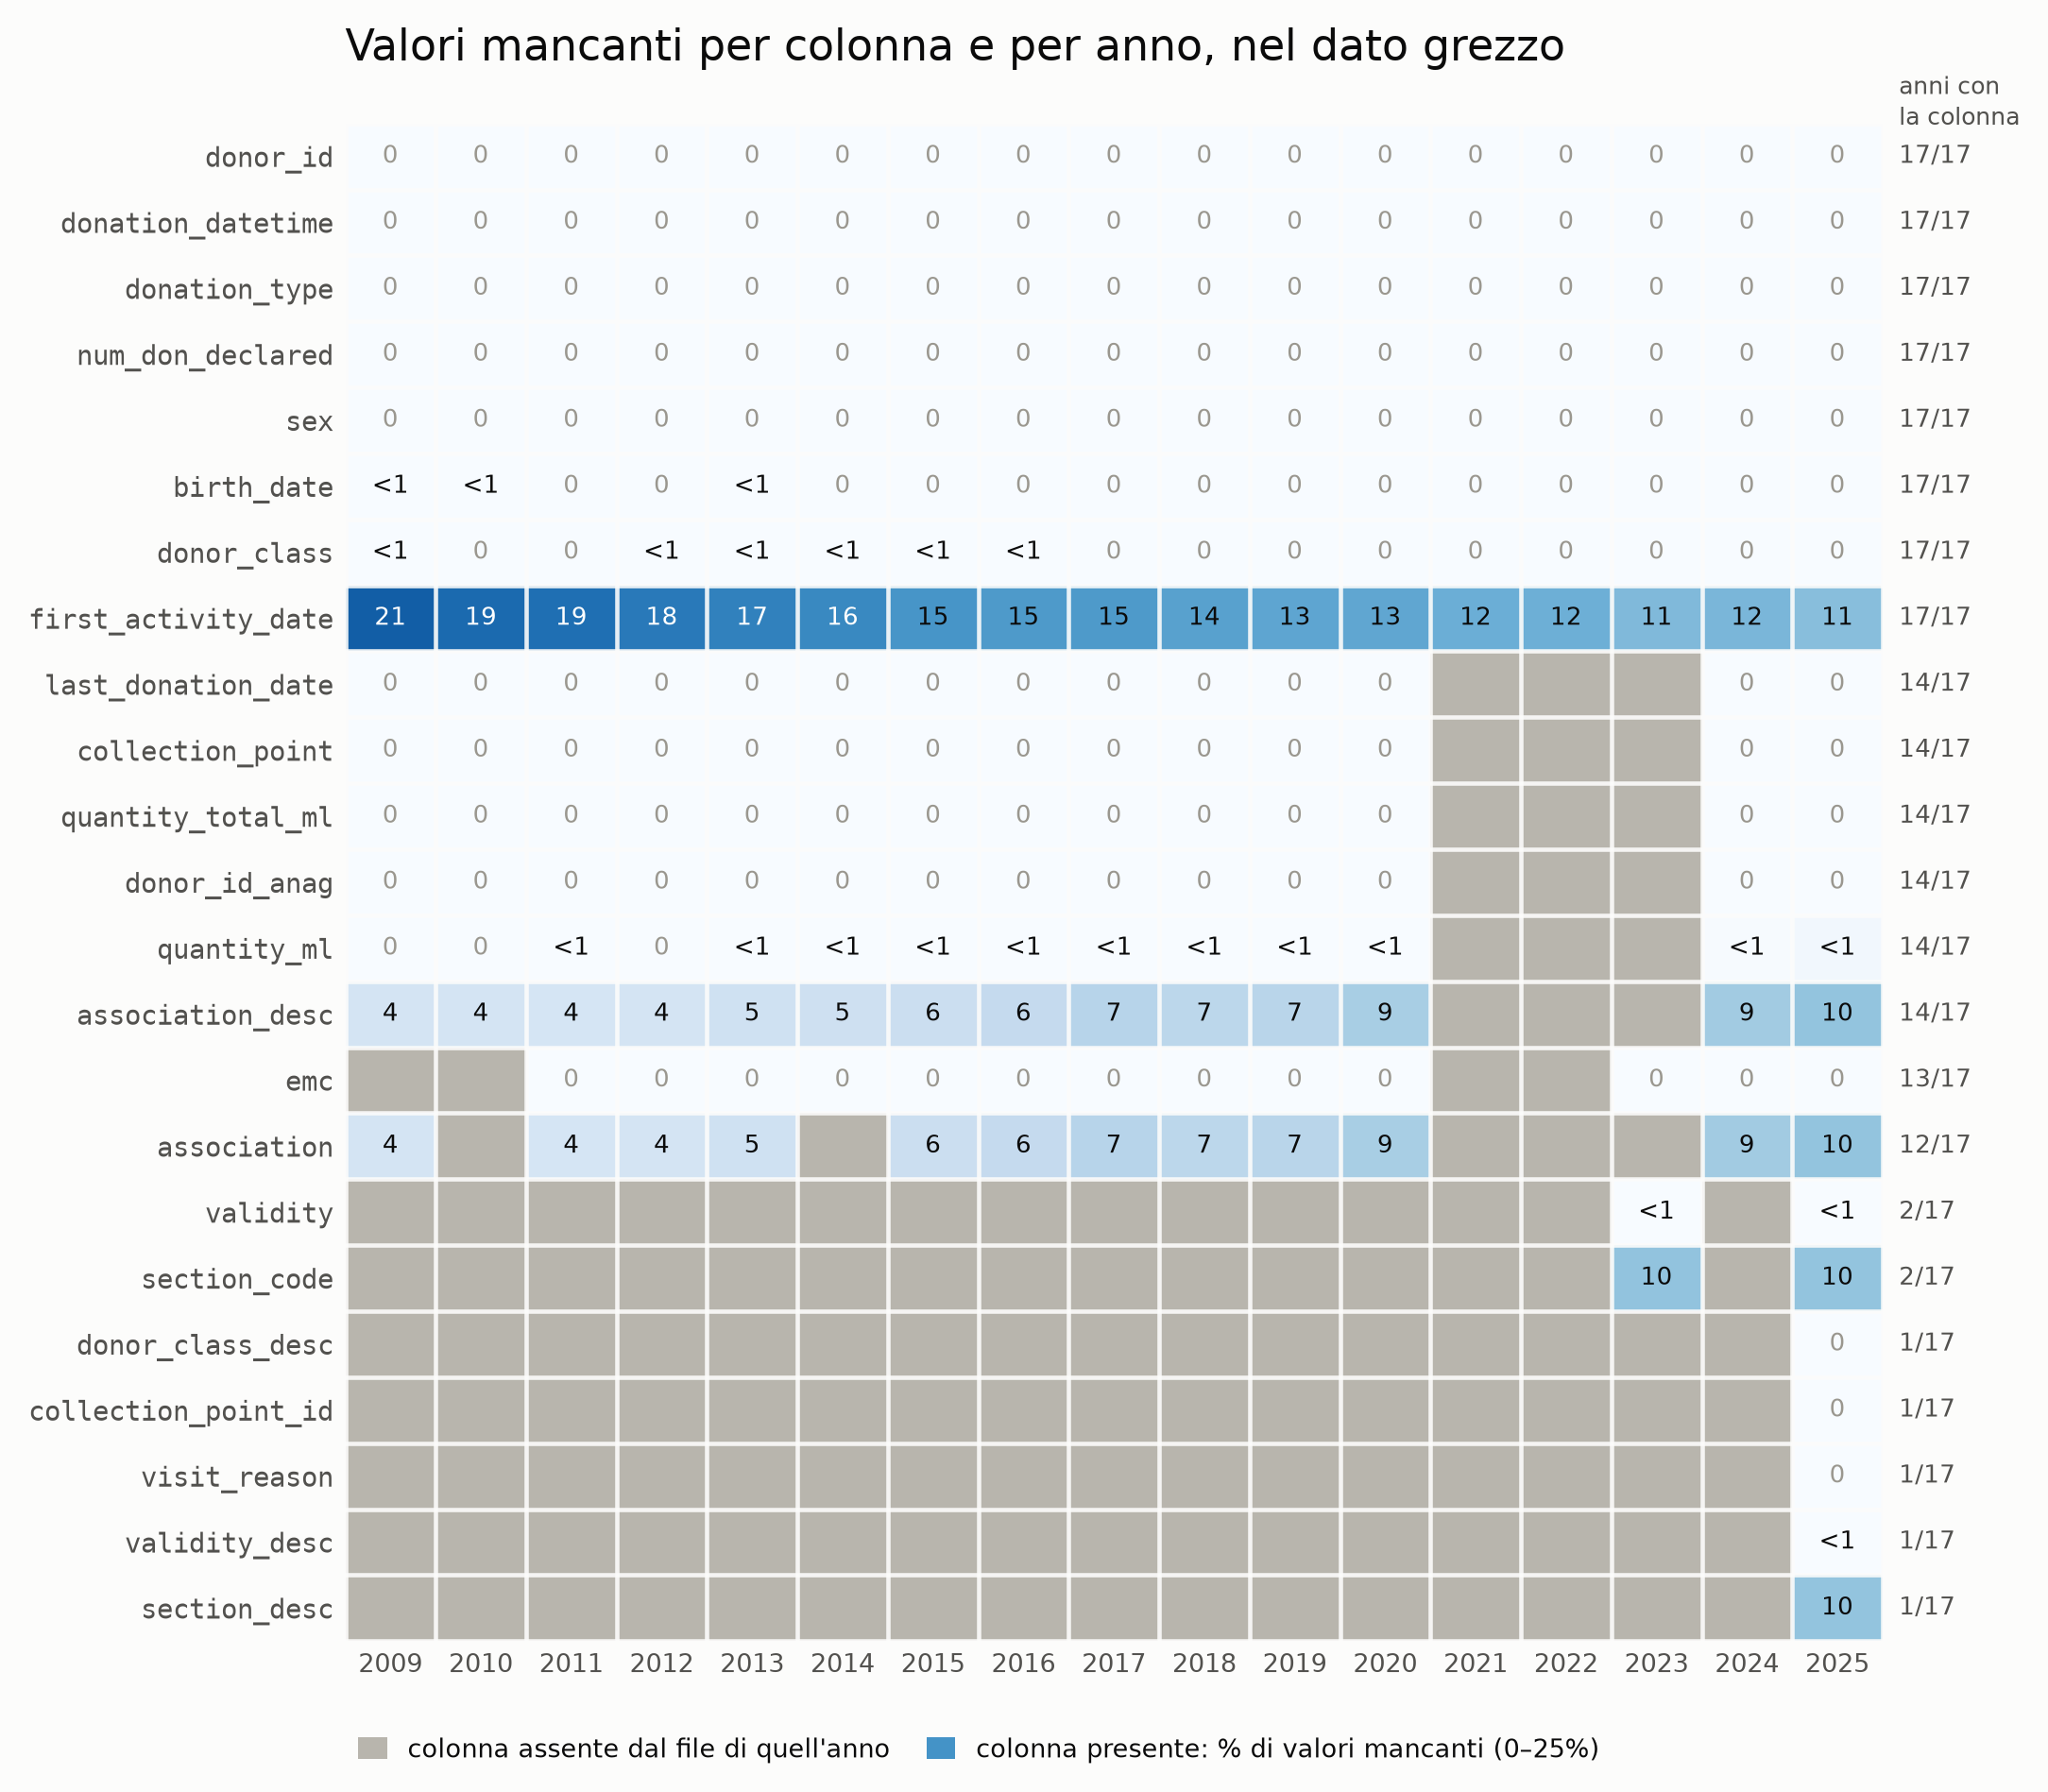
\includegraphics[width=0.95\linewidth]{img/fig_null_heatmap.png}
    \caption{Valori mancanti per colonna e per anno nei file sorgente, prima
    di qualsiasi elaborazione. Il grigio indica una colonna che in quell'anno
    non esiste affatto; dove la colonna esiste, il numero è la percentuale di
    valori mancanti e l'intensità del blu vi è proporzionale. Le due
    condizioni sono tenute separate perché dicono cose diverse: la prima è una
    proprietà del tracciato, la seconda del dato.}
    \label{fig:null_heatmap}
\end{figure}

% ───────────────────────────────────────────────────────────────────────
\section{Due decisioni che condizionano tutto il resto}
\label{sec:decisioni}

\paragraph{Quale colonna identifica il donatore.}
I file contengono due identificativi anonimi, \texttt{crd} e \texttt{id\_anag}.
Solo il primo è presente in \textbf{tutti e 27 i file}; il secondo manca nei
file 2021, 2022 e in entrambi i file 2023. La corrispondenza fra i due è di
fatto biunivoca: su 41\,201 valori distinti di \texttt{crd}, soltanto
\textbf{tre} sono associati a più di un \texttt{id\_anag}, e nessun
\texttt{id\_anag} è associato a più di un \texttt{crd}.

La scelta ricade quindi su \texttt{crd}:
adottare \texttt{id\_anag} costringe a ricostruire l'identità del donatore per
il triennio 2021--2023 con una mappatura di copertura parziale, e ogni donatore
non mappato risulta artificialmente nuovo in quegli anni --- con effetti
diretti sul conteggio dei nuovi ingressi del \cref{ch:eda} e sulle coorti del
\cref{ch:retention}. Con \texttt{crd} il problema non si pone.

\paragraph{L'inizio dell'attività da donatore è un importante predittore.}
La colonna \texttt{dtinizatt\_da} registra quando il soggetto ha cominciato a
donare, anche molto prima dell'inizio della finestra osservata. È \textbf{nulla
su 54\,017 righe}, e la sua compilazione dipende dalla prassi
della sede.

\begin{table}[ht]
\centering
\caption{Quota di righe prive di data di inizio attività, per punto di
raccolta. La compilazione è una prassi locale, non un attributo del donatore.}
\label{tab:nulli_sede}
\begin{tabular}{@{}lrr@{}}
\toprule
\textbf{Punto di raccolta} & \textbf{Righe} & \textbf{Senza data di inizio} \\
\midrule
Maggiore (Trieste)  & 152\,302 & \phantom{0}2{,}3\% \\
Burlo (Trieste)     & \phantom{0}12\,353 & \phantom{0}1{,}2\% \\
Autoemoteca TS      & \phantom{00}7\,091 & \phantom{0}0{,}3\% \\
Autoemoteca UD      & \phantom{00}3\,034 & 17{,}9\% \\
Autoemoteca GO      & \phantom{0}25\,475 & 23{,}0\% \\
Monfalcone S.\ Polo & \phantom{0}47\,601 & 29{,}2\% \\
Sede Gorizia        & \phantom{0}49\,727 & \textbf{45{,}7\%} \\
Cormons             & \phantom{000}533 & 49{,}2\% \\
Grado               & \phantom{00}1\,070 & 52{,}0\% \\
\midrule
Non registrato (2021--2023) & \phantom{0}54\,485 & 12{,}0\% \\
\bottomrule
\end{tabular}
\end{table}

A Trieste il campo è quasi sempre valorizzato, nell'Isontino spesso no
(\cref{tab:nulli_sede}). Ne segue che \textbf{scartare le righe prive di quel
campo equivale a cancellare in larga parte una provincia}: delle donazioni che
andrebbero perse, oltre tre quarti sono di Gorizia e Monfalcone. Il campo viene
quindi conservato come covariata, e dove manca resta mancante --- l'evento di
donazione, che è osservato senza ambiguità, non si butta. L'effetto sulla
geografia è discusso nella \cref{sec:collection}.

% ───────────────────────────────────────────────────────────────────────
\section{La pipeline}
\label{sec:cleaning}

La pipeline è organizzata in \textbf{quattro stadi} (\cref{fig:pipeline}). Ogni
stadio legge il file prodotto da quello precedente e ne scrive uno nuovo:
nessuno riscrive il proprio input, quindi ogni comando è rieseguibile senza
effetti d'ordine e una rielaborazione parziale non lascia il dataset in uno
stato intermedio.

\begin{figure}[H]
    \centering
    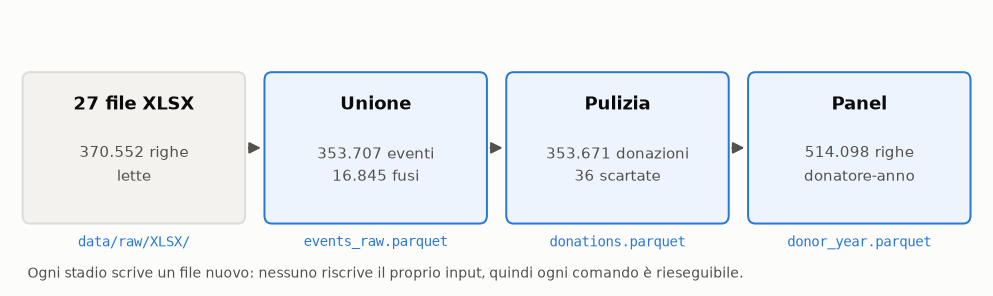
\includegraphics[width=\linewidth]{img/fig_pipeline_diagram.png}
    \caption{I quattro stadi della pipeline, con il numero di righe in uscita
    da ciascuno.}
    \label{fig:pipeline}
\end{figure}

\paragraph{Stadio 1 --- Unione.}
I 27 file vengono ricondotti allo schema comune e uniti. I due file 2023
meritano una nota: contengono \emph{lo stesso insieme di eventi} (16\,843 righe
ciascuno, chiavi coincidenti) e differiscono per una sola colonna,
\texttt{sez} nell'uno e \texttt{validita} nell'altro. Caricarli entrambi
raddoppierebbe l'anno; caricarne uno solo butterebbe via una colonna. Vengono
quindi \emph{fusi} sulla chiave dell'evento, conservando entrambe le colonne:
le 33\,686 righe dei due file si riducono a \textbf{16\,842 eventi} distinti.
La fusione è l'unica riduzione di questo stadio --- a essa si aggiunge una sola
riga, un duplicato interno al file 2024 --- per un totale di
\textbf{16\,845 righe} in meno, elencate una per una in un report di
riconciliazione.

\paragraph{Stadio 2 --- Pulizia.}
Ogni regola è una funzione separata che dichiara quante righe tocca. Le regole
applicate sono: normalizzazione delle date; filtro sull'età ammissibile
(18--90 anni, dove i valori oltre soglia sono errori evidenti di data di
nascita); consolidamento dei punti di raccolta, che nei file identificano il
singolo veicolo o turno e non la sede (\emph{Autoemoteca GO}, \emph{Seconda
autoemoteca GO}, \ldots) e vengono ricondotti a nove sedi; normalizzazione dei
codici di associazione, che si riducono a nove livelli.

Le tipologie di donazione minoritarie e le descrizioni di associazione
\emph{non} vengono invece accorpate in questo stadio: restano tutti i dieci
codici di tipologia e tutte le tredici descrizioni presenti nei file grezzi. Il
raggruppamento in una categoria residuale avviene, dove serve, a valle: nel
\cref{ch:glm} la tipologia prevalente pregressa usa una categoria
\textsc{altro} per i codici sotto soglia.

\paragraph{Stadio 3 --- Panel donatore-anno.}
L'ultimo stadio non pulisce: cambia unità di osservazione. Per ogni donatore si
costruisce una riga per \emph{ogni} anno dal suo ingresso in poi, anche per gli
anni in cui non ha donato. Gli anni a zero sono \textbf{il 63{,}9\%} delle
righe, e senza di essi l'abbandono --- l'evento che il \cref{ch:retention}
studia e che il \cref{ch:glm} vuole modellare --- semplicemente non
comparirebbe nei dati. La somma della risposta su un anno è, per costruzione,
il totale di quell'anno: aggregato e individuale non possono contraddirsi.

L'\cref{alg:panel} riassume la costruzione. Due dettagli non sono cosmetici. Il
primo è la riga~3: gli attributi del donatore si prendono alla \emph{prima}
riga osservata e non all'ultima, altrimenti in ogni anno del panel comparirebbe
informazione raccolta dopo. Il secondo è la riga~9, l'unica verifica che conta
davvero: se la somma della risposta non coincide con il numero di donazioni di
partenza, la costruzione si ferma.

\begin{algorithm}[H]
\caption{Costruzione del panel donatore-anno}
\label{alg:panel}
\begin{algorithmic}[1]
\Require eventi di donazione $D$; ultimo anno della finestra $T$
\Ensure panel $P$ con una riga per coppia (donatore, anno)
\State $A \gets$ conteggio di $D$ per (donatore, anno)
\Comment{solo gli anni in cui si è donato}
\State per ogni donatore $i$: attributi $x_i \gets$ valori della sua prima riga
osservata \Comment{mai dell'ultima: sarebbe informazione futura}
\State per ogni donatore $i$: $e_i \gets \min\{\,t : (i,t) \in A\,\}$
\Comment{anno d'ingresso}
\State $P \gets \{\,(i, t) : e_i \le t \le T\,\}$
\Comment{griglia densa: anche gli anni senza donazioni}
\State $y_{it} \gets A[i,t]$ se presente, altrimenti $0$
\Comment{è qui che nascono gli zeri}
\State $\text{carriera}_{it} \gets t - e_i$; \ \ $\text{età}_{it} \gets t -
\text{anno di nascita}_i$
\State unisci $x_i$ a ogni riga di $P$
\If{$\sum_{i,t} y_{it} \neq |D|$} \State \textbf{interrompi}
\Comment{il panel deve rendere conto di ogni donazione}
\EndIf
\State \Return $P$
\end{algorithmic}
\end{algorithm}

\begin{table}[H]
\centering
\small
\caption{Simboli dell'\cref{alg:panel} e valori sul dataset finale.}
\label{tab:panel_simboli}
\begin{tabularx}{\linewidth}{@{}l X l@{}}
\toprule
\textbf{Simbolo} & \textbf{Significato} & \textbf{Valore} \\
\midrule
$D$ & eventi di donazione del dataset pulito, uno per riga & --- \\
$|D|$ & numero di eventi & 353\,671 \\
$T$ & ultimo anno della finestra osservata & 2025 \\
$i$ & donatore & 43\,299 distinti \\
$t$ & anno solare & $e_i,\dots,T$ \\
$A$ & conteggi per (donatore, anno), solo per gli anni con almeno una donazione & --- \\
$A[i,t]$ & donazioni del donatore $i$ nell'anno $t$ & --- \\
$x_i$ & attributi fissi del donatore (genere, anno di nascita, \ldots), presi dalla prima riga osservata & --- \\
$e_i$ & anno d'ingresso: primo anno con una donazione & 2009--2025 \\
$P$ & panel: una riga per ogni coppia $(i,t)$ con $e_i \le t \le T$ & 514\,098 righe \\
$y_{it}$ & risposta: donazioni di $i$ nell'anno $t$, zero se non ha donato & 63{,}9\% di zeri \\
$\text{carriera}_{it}$ & anni trascorsi dall'ingresso, $t - e_i$ & $0,\dots,16$ \\
$\text{età}_{it}$ & età nell'anno $t$ & --- \\
\bottomrule
\end{tabularx}
\end{table}

\subsection{Bilancio quantitativo}
\label{sec:phaselog}

\begin{table}[ht]
\centering
\caption{Bilancio riga-per-riga della pipeline.}
\label{tab:cleaninglog}
\begin{tabular}{@{}llrr@{}}
\toprule
\textbf{Stadio} & \textbf{Operazione} & \textbf{Righe in uscita} & \textbf{Variazione} \\
\midrule
0 & Lettura dei 27 file          & 370\,552 & ---          \\
1 & Fusione degli eventi doppi   & 353\,707 & $-16\,845$   \\
2 & Regole di pulizia            & 353\,671 & $-36$        \\
3 & Panel donatore $\times$ anno & 514\,098 & (cambio di unità) \\
\bottomrule
\end{tabular}
\end{table}

Il bilancio \textbf{chiude a zero}: ogni riga letta o esce nel file finale o
compare, con la ragione, in uno dei due report di riconciliazione. Le regole di
pulizia scartano \textbf{36 righe su 370\,552}, meno di un decimillesimo: è la
conseguenza diretta della scelta della \cref{sec:decisioni} di non usare la
completezza di un campo amministrativo come criterio di ammissione.

% ───────────────────────────────────────────────────────────────────────
\section{Struttura del dataset finale}
\label{sec:dataset}

Il dataset di eventi contiene \textbf{353\,671 righe}, una per donazione,
relative a \textbf{43\,299 donatori distinti} nel periodo 2009--2025. La chiave
naturale è la tripla (\texttt{donor\_id}, \texttt{donation\_datetime},
\texttt{donation\_type}). Il panel derivato ne conta \textbf{514\,098}, una per
coppia donatore-anno.

\small
\setlength{\tabcolsep}{4pt}
\begin{longtable}{@{}llp{7.6cm}@{}}
\caption{Dizionario delle variabili del dataset di eventi.}
\label{tab:columns} \\
\toprule
\textbf{Colonna} & \textbf{Tipo} & \textbf{Descrizione} \\
\midrule
\endfirsthead
\multicolumn{3}{l}{\textit{(continua dalla pagina precedente)}} \\
\toprule
\textbf{Colonna} & \textbf{Tipo} & \textbf{Descrizione} \\
\midrule
\endhead
\midrule
\multicolumn{3}{r}{\textit{(continua nella pagina seguente)}} \\
\endfoot
\bottomrule
\endlastfoot
\texttt{donor\_id}             & stringa  & Identificativo anonimo (\texttt{crd}) \\
\texttt{donation\_datetime}    & datetime & Data e ora dell'evento \\
\texttt{donation\_year}        & int      & Anno dell'evento \\
\texttt{donation\_month}       & int      & Mese dell'evento (1--12) \\
\texttt{donation\_type}        & stringa  & Tipo (\textsc{sangue}, \textsc{plasmaf}, \ldots) \\
\texttt{sex}                   & stringa  & Sesso (M / F) \\
\texttt{birth\_date}           & data     & Data di nascita \\
\texttt{age}                   & int      & Età al momento della donazione \\
\texttt{donor\_class}          & stringa  & Classe donatore (P, O, D, A) \\
\texttt{donor\_class\_regime}  & stringa  & Regime di codifica della classe (\cref{sec:glm_effects}) \\
\texttt{association}           & stringa  & Codice associazione \\
\texttt{association\_desc}     & stringa  & Nome associazione \\
\texttt{collection\_point}     & stringa  & Sede di raccolta consolidata \\
\texttt{first\_activity\_date} & data     & Inizio dell'attività donazionale \\
\texttt{last\_donation\_date}  & data     & Ultima donazione registrata \\
\texttt{quantity\_ml}          & float    & Quantità donata nell'evento (mL) \\
\texttt{validity}              & stringa  & Validità dichiarata (in 4 file su 27) \\
\texttt{num\_don\_declared}    & int      & Conteggio dichiarato --- \emph{solo controllo} \\
\texttt{quantity\_total\_ml}   & float    & Quantità cumulativa --- \emph{solo controllo} \\
\texttt{donor\_id\_anag}       & stringa  & Identificativo alternativo --- \emph{solo controllo} \\
\end{longtable}

\paragraph{Due colonne non esplicative.}
\texttt{num\_don\_declared} e \texttt{quantity\_total\_ml} sono conservate
soltanto come controllo e non compaiono in nessun modello. La prima non è un
attributo dell'evento ma un aggregato di livello superiore --- il numero di
donazioni del gruppo (donatore, anno, tipologia) --- replicato su ciascuna riga
del gruppo; coincide con il conteggio osservabile nel $96{,}1\%$ dei casi. La
seconda è la somma delle quantità nello stesso gruppo, quindi è la risposta
moltiplicata per un volume medio. \textbf{Il conteggio delle donazioni si
ottiene sempre contando le righe.} Il punto è ripreso nella
\cref{sec:glm_unit}, dove ha conseguenze dirette sulla specifica del modello.

\paragraph{Donazioni dichiarate non valide.}
La colonna \texttt{validity} esiste solo in 4 file su 27 e marca 752 donazioni
come non valide. Non essendo applicabile in modo uniforme all'intero periodo,
non viene usata come filtro: quelle righe restano nel conteggio, e la variante
che le esclude è stata verificata come analisi di sensitività senza effetti
apprezzabili sui risultati dei capitoli seguenti.

% ───────────────────────────────────────────────────────────────────────
\section{Sintesi del capitolo}
\label{sec:datasummary}

Il dataset analitico finale contiene \textbf{353\,671 eventi di donazione}
relativi a \textbf{43\,299 donatori} osservati fra il 2009 e il 2025, ottenuti
da 27 file Excel attraverso quattro stadi, ciascuno dei quali produce un file
nuovo e un bilancio verificabile. La riduzione complessiva rispetto al dato
grezzo è di 16\,881 righe, quasi interamente dovuta alla fusione delle due
estrazioni del 2023.

Le due decisioni che pesano di più --- usare \texttt{crd} come identificativo e
trattare la data di inizio attività come covariata anziché come requisito ---
sono quelle che determinano quanto dato arriva alle analisi. La seconda in
particolare ha un effetto geografico: valutarla diversamente significa
raccontare l'Isontino con circa la metà delle sue donazioni.

% ══════════════════════════════════════════════════════════════════════════════
%  Fine Capitolo — Dati e Costruzione del Dataset
% ══════════════════════════════════════════════════════════════════════════════
